\chapter{CƠ SỞ LÍ THUYẾT}

\section{Tổng quan về ảnh y tế trong chẩn đoán bệnh lý cột sống}
Chẩn đoán hình ảnh đóng vai trò then chốt trong việc xác định nguyên nhân và đánh giá mức độ nghiêm trọng của các bệnh lý cột sống. Việc lựa chọn phương pháp hình ảnh phù hợp phụ thuộc vào tình trạng lâm sàng và cấu trúc giải phẫu cần khảo sát.

\subsection{Các loại bất thường thường gặp trên ảnh MRI thắt lưng}
Trước khi đi vào chi tiết kĩ thuật, phần này tóm tắt các loại bất thường mà mô hình AI cần phát hiện trên ảnh MRI cột sống thắt lưng. Các bất thường được chia theo cấu trúc giải phẫu bị ảnh hưởng:

\textbf{Bất thường ở đĩa đệm:}
\begin{itemize}
    \item \textbf{Thoái hóa đĩa đệm (Thang đo Pfirrmann grade 1-5)~\cite{pfirrmann2001grading}:} đĩa đệm mất nước, giảm chiều cao, tín hiệu T2 giảm dần.
    \item \textbf{Thoát vị đĩa đệm (Disc herniation):} nhân nhầy bị đẩy ra ngoài vòng sợi, chèn ép vào tủy sống hoặc rễ thần kinh.
    \item \textbf{Phồng đĩa đệm (Disc bulging):} dạng nhẹ hơn của thoát vị, vành đĩa đệm phình đều ra ngoài.
    \item \textbf{Hẹp đĩa đệm (Disc narrowing):} giảm chiều cao đĩa đệm so với bình thường.
\end{itemize}

\textbf{Bất thường ở đốt sống :}
\begin{itemize}
    \item \textbf{Trượt đốt sống (Spondylolisthesis):} một đốt sống trượt ra trước hoặc sau so với đốt sống liền kề.
    \item \textbf{Tổn thương endplate (Upper/Lower endplate damage):} các vết nứt hoặc schmorl node ở mặt trên hoặc dưới của đốt sống.
    \item \textbf{Biến đổi modic (Modic changes type 1--3)~\cite{modic1988degenerative}:} biến đổi tủy xương dưới sụn endplate, biểu hiện rõ trên T1 và T2.
\end{itemize}

\textbf{Bất thường ở ống sống và lỗ liên hợp:}
\begin{itemize}
    \item \textbf{Hẹp ống sống (Spinal canal stenosis):} thu hẹp ống sống do thoái hóa, thoát vị hoặc dày dây chằng vàng.
    \item \textbf{Hẹp lỗ liên hợp (Neural foraminal narrowing - trái và phải):} thu hẹp lỗ thoát rễ thần kinh ra khỏi cột sống.
    \item \textbf{Hẹp ngách bên (Subarticular/lateral recess stenosis - trái và phải):} thu hẹp vùng ngách bên ống sống, nơi rễ thần kinh đi qua trước khi vào lỗ liên hợp.
\end{itemize}

Báo cáo tập trung tinh chỉnh mô-đun grading cho 3 nhãn theo chuẩn RSNA 2024~\cite{rsna2024dataset} (canal stenosis, foraminal narrowing trái/phải) và mở rộng lên 8 nhãn theo chuẩn SPIDER~\cite{vansluijs2022spider} (thêm Pfirrmann, Modic, narrowing, spondylolisthesis, endplate, herniation, bulging). Hình~\ref{fig:abnormality_examples} minh họa sự khác biệt trực quan giữa case Normal/Mild và Severe cho 3 conditions chính trên ảnh MRI Sagittal T2/STIR.

\begin{figure}[H]
    \centering
    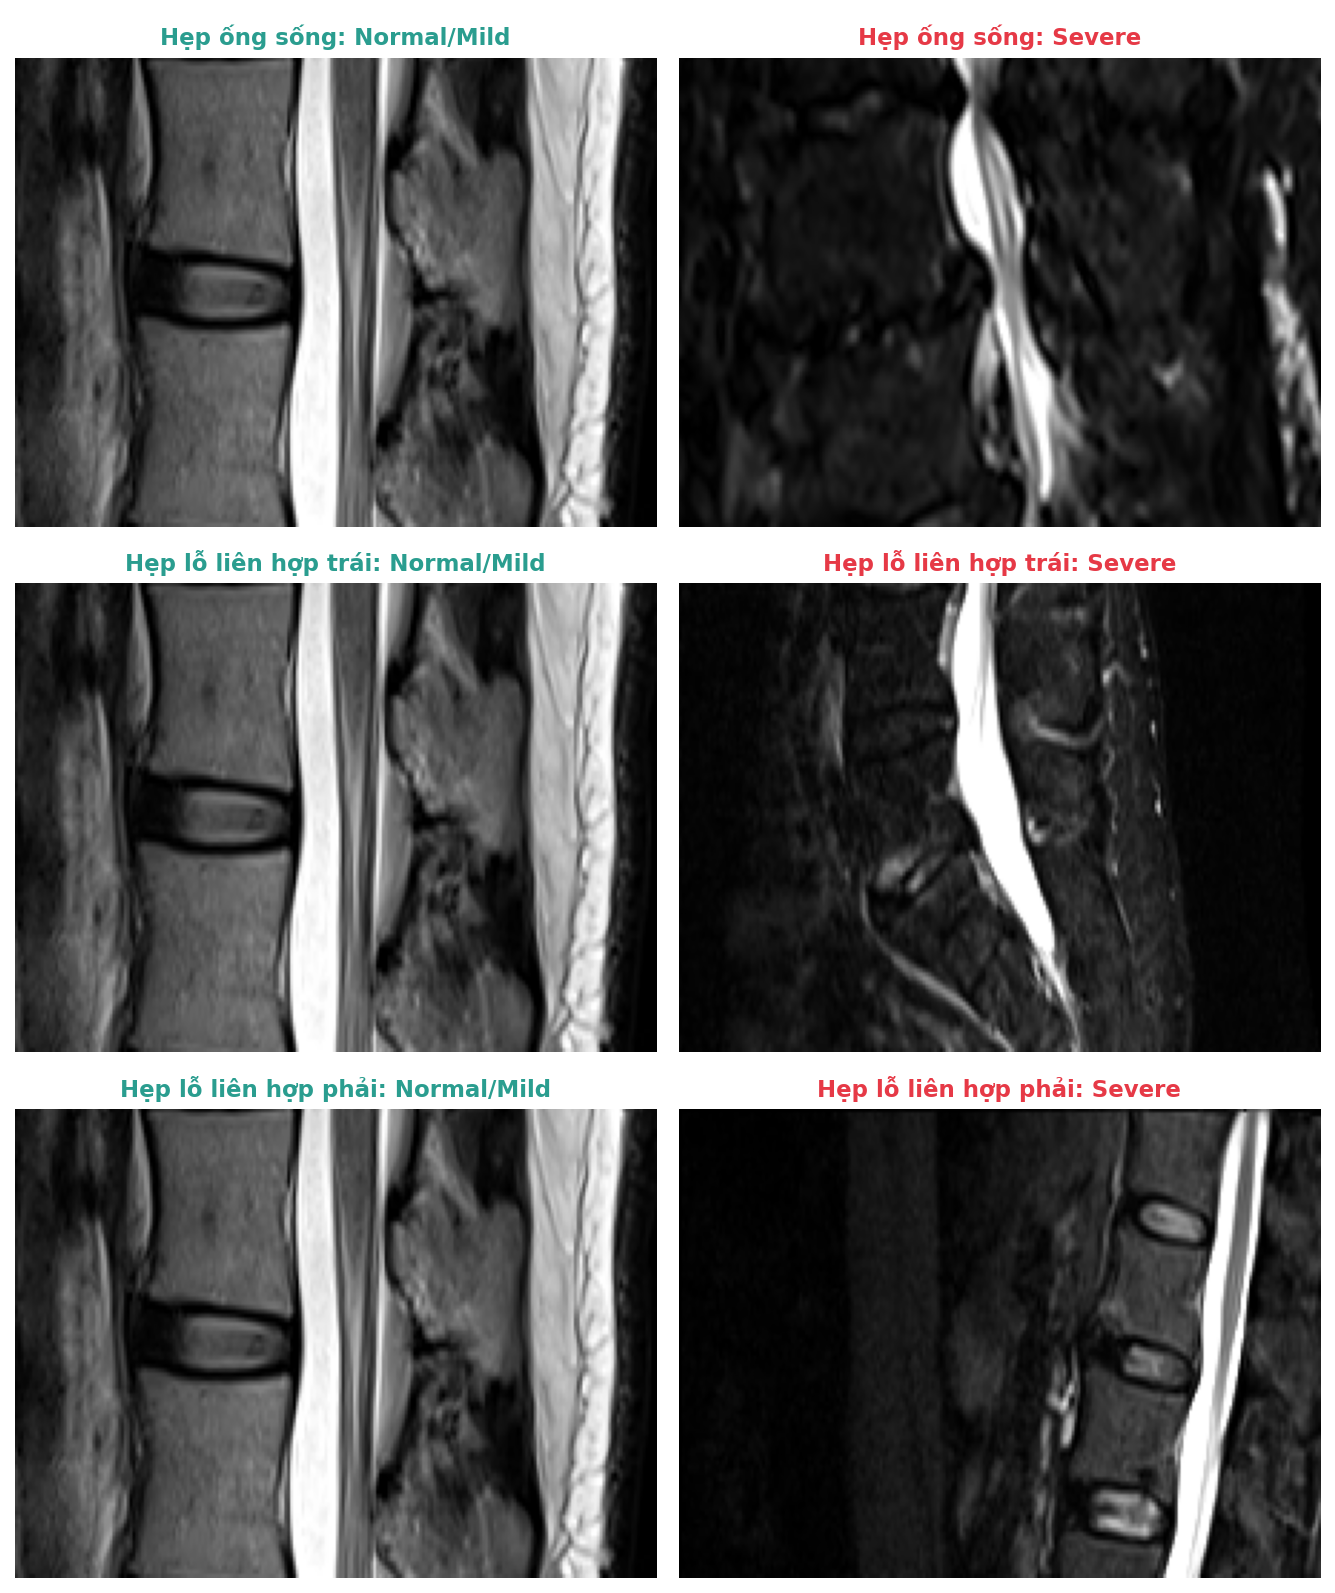
\includegraphics[width=0.85\textwidth]{cslt/abnormality_examples.png}
    \caption{Ví dụ Normal/Mild vs Severe cho 3 conditions RSNA.}
    \label{fig:abnormality_examples}
\end{figure}

% Hình~\ref{fig:spider_abnormality_examples} bổ sung minh họa cho 4 loại bất thường ở đĩa đệm và đốt sống từ SPIDER dataset, bao gồm Pfirrmann grade, thoát vị đĩa đệm, phồng đĩa đệm và trượt đốt sống.

% \begin{figure}[H]
%     \centering
%     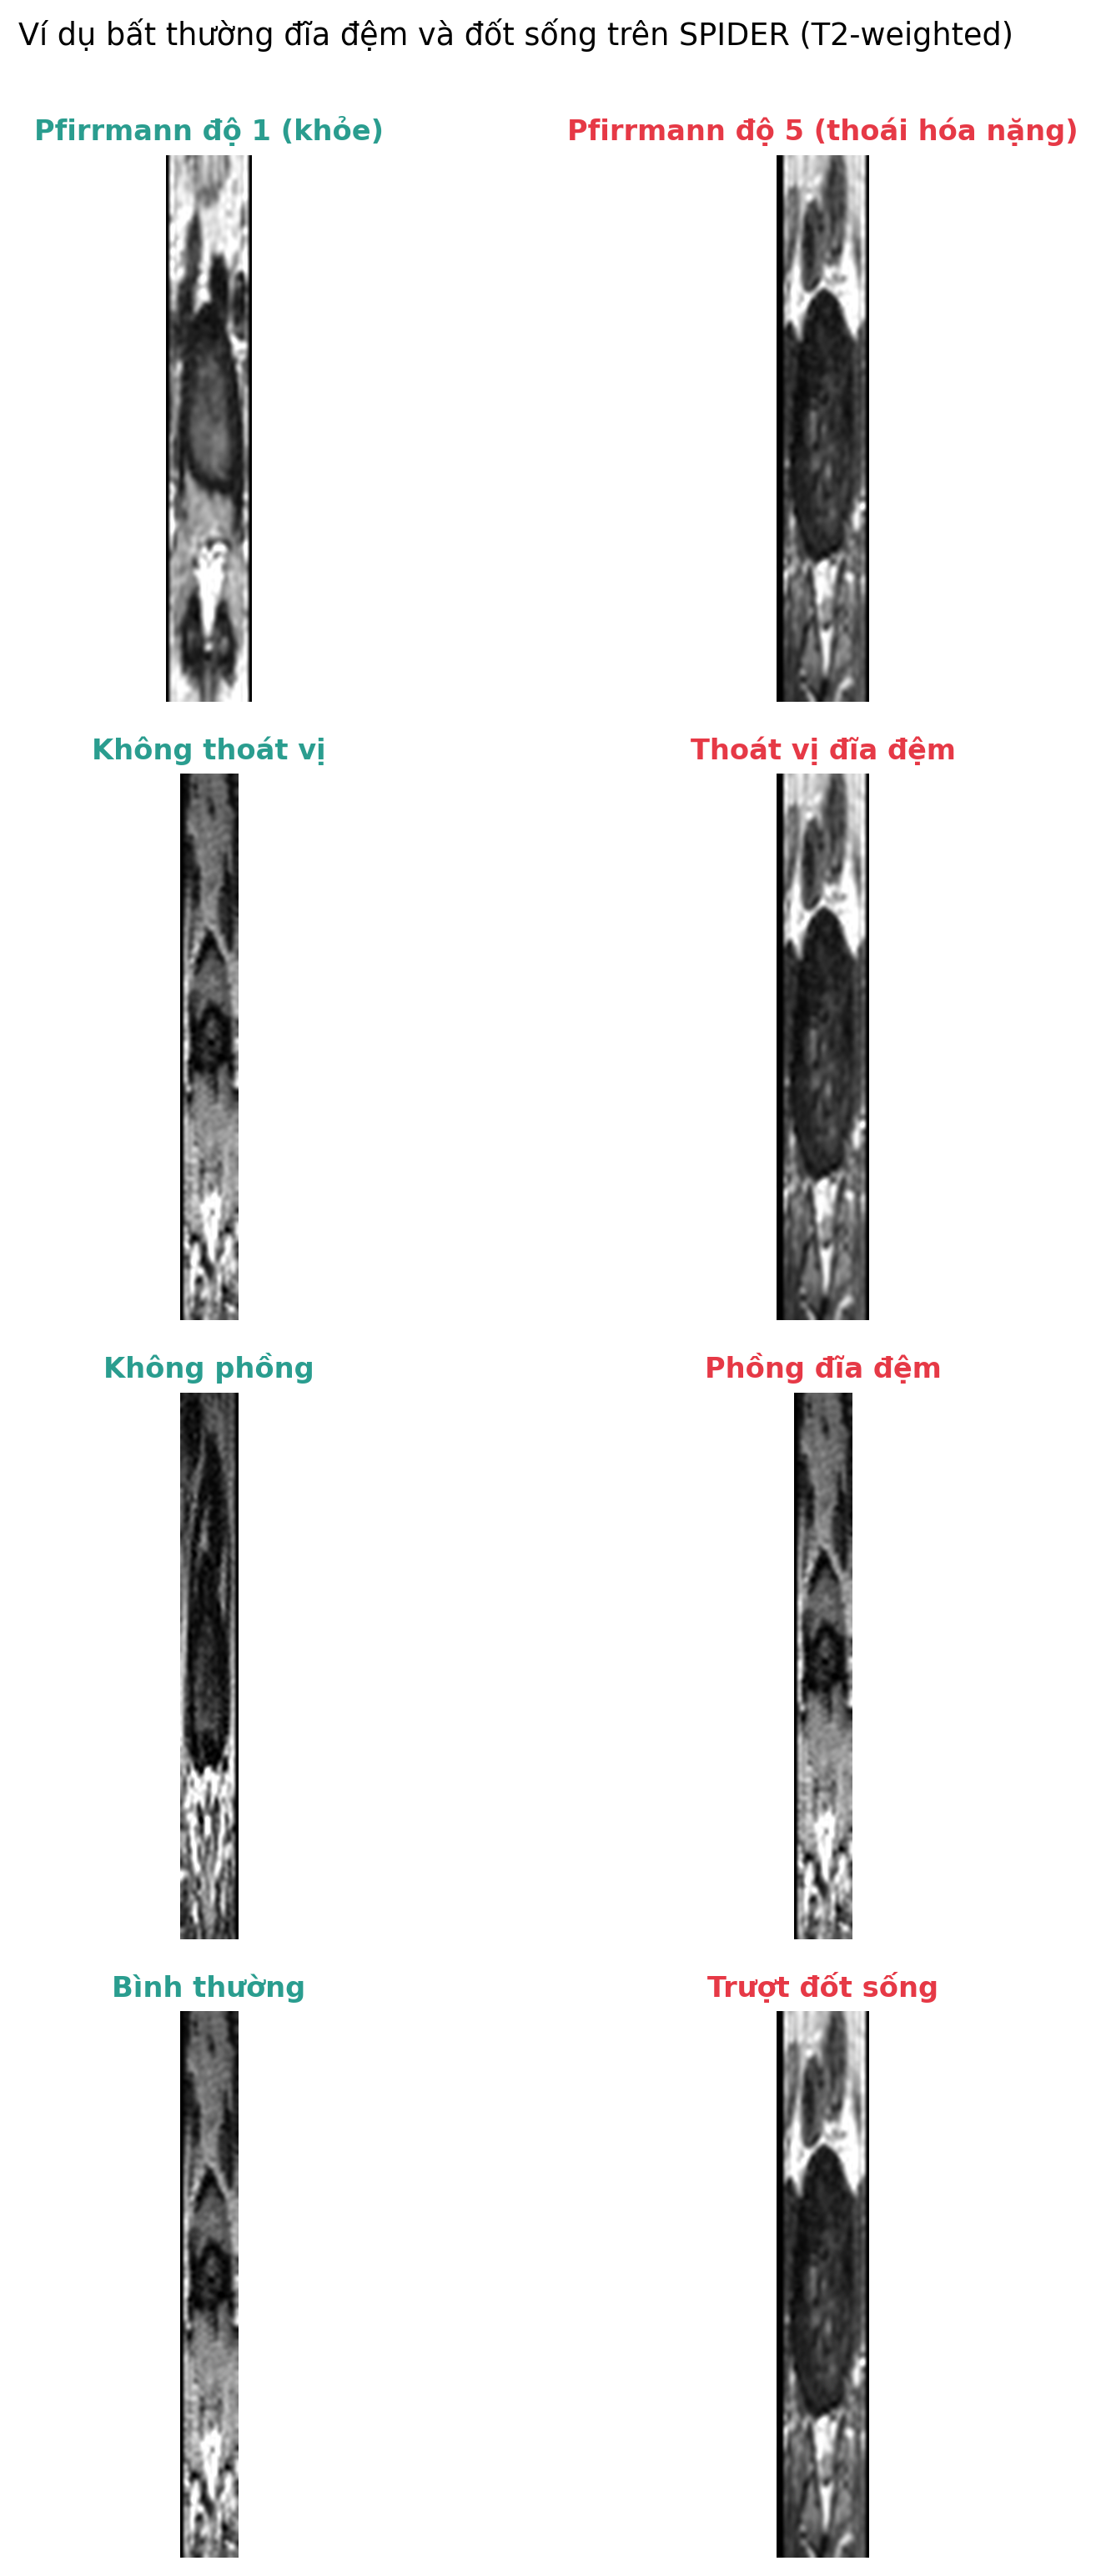
\includegraphics[width=0.75\textwidth]{cslt/spider_abnormality_examples.png}
%     \caption{Bất thường đĩa đệm và đốt sống trên SPIDER.}
%     \label{fig:spider_abnormality_examples}
% \end{figure}

\subsection{Các mặt cắt MRI và hướng chụp cơ bản}
Một khối ảnh MRI cột sống 3D có thể được trình bày dưới ba mặt cắt chính, mỗi mặt cắt phù hợp cho việc đánh giá các cấu trúc khác nhau:

\begin{itemize}
    \item \textbf{Mặt cắt dọc giữa (Sagittal):} cắt theo mặt phẳng đứng trước-sau, chia cơ thể thành hai nửa trái-phải. Đây là mặt cắt \emph{quan trọng nhất} cho việc đánh giá thoái hóa đĩa đệm, thoát vị, và sắp xếp tổng thể của cột sống. Trên ảnh Sagittal T2-weighted, đĩa đệm khỏe có tín hiệu cao (sáng), tủy sống và CSF nổi bật rõ. Báo cáo này sử dụng chủ yếu các lát cắt sagittal làm input cho mô hình.
    \item \textbf{Mặt cắt ngang (Axial):} cắt theo mặt phẳng ngang, vuông góc với trục cột sống. Đây là mặt cắt tốt nhất để đánh giá hẹp ống sống, hẹp ngách bên, và quan sát mối quan hệ giữa đĩa đệm với rễ thần kinh hai bên. SpineNetV2 baseline chưa khai thác mặt cắt này, đây là một hướng phát triển trong tương lai (xem Chương 6).
    \item \textbf{Mặt cắt trán (Coronal):} cắt theo mặt phẳng đứng song song với lưng. Mặt cắt này ít dùng cho chẩn đoán đĩa đệm nhưng hữu ích cho việc đánh giá vẹo cột sống (scoliosis) và sắp xếp các đốt sống.
\end{itemize}

Với mỗi mặt cắt, dữ liệu MRI thường có hai chuỗi xung phổ biến:
\begin{itemize}
    \item \textbf{T1-weighted (T1):} hiển thị mô mỡ sáng, dịch tối. Dùng để đánh giá cấu trúc giải phẫu chi tiết và phát hiện biến đổi Modic type 1 (giảm tín hiệu).
    \item \textbf{T2-weighted (T2) / STIR:} hiển thị dịch sáng, mô mỡ tối hơn. Đây là chuỗi xung chính cho phát hiện viêm, phù nề, thoát vị đĩa đệm và đánh giá Pfirrmann.
\end{itemize}

\subsection{Các loại ảnh y tế thường dùng}
\textbf{X-quang (X-ray):} Là kỹ thuật cơ bản và phổ biến nhất, sử dụng tia X để tạo ra hình ảnh hai chiều của xương. X-quang rất hữu ích để đánh giá cấu trúc tổng thể của cột sống, phát hiện các vấn đề như gãy xương, trượt đốt sống, vẹo cột sống, hoặc các thay đổi thoái hóa ở xương. Tuy nhiên, X-quang có hạn chế trong việc hiển thị các mô mềm như đĩa đệm, tủy sống hay dây thần kinh.\\
    
\textbf{Cắt lớp vi tính (Computed Tomography - CT):} Kỹ thuật này cũng sử dụng tia X nhưng kết hợp với xử lý máy tính để tạo ra các hình ảnh cắt lớp ngang chi tiết của cơ thể. CT cho thấy hình ảnh xương với độ phân giải rất cao, vượt trội hơn X-quang trong việc phát hiện các gãy xương phức tạp, hẹp ống sống do xương hoặc các khối u xương. Mặc dù có thể thấy được mô mềm tốt hơn X-quang, CT vẫn không chi tiết bằng MRI.\\
    
 \textbf{Cộng hưởng từ (Magnetic Resonance Imaging - MRI):} Được xem là tiêu chuẩn vàng trong chẩn đoán các bệnh lý liên quan đến mô mềm của cột sống. MRI sử dụng từ trường mạnh và sóng radio để tạo ra hình ảnh cắt lớp chi tiết. Kỹ thuật này khảo sát xuất sắc các cấu trúc như đĩa đệm (phát hiện thoát vị), tủy sống, rễ thần kinh, dây chằng và các khối u mô mềm. MRI là công cụ không thể thiếu để chẩn đoán chính xác nguyên nhân gây chèn ép thần kinh.

\subsection{Các định dạng tệp ảnh y tế phổ biến}
Trong lĩnh vực chẩn đoán hình ảnh, dữ liệu được lưu trữ dưới nhiều định dạng khác nhau, mỗi định dạng có những đặc điểm riêng về cấu trúc và ứng dụng. Hai trong số các định dạng phổ biến nhất trong nghiên cứu và lâm sàng là DICOM và NIfTI; Bảng~\ref{tab:file_formats} tóm tắt đặc điểm của hai định dạng này.

\begin{table}[h!]
\centering
\caption{Tóm tắt đặc điểm của các định dạng tệp ảnh y tế.}
\label{tab:file_formats}
\begin{tabular}{|l|p{4cm}|l|p{5cm}|}
\hline
\textbf{Định dạng} & \textbf{Header} & \textbf{Phần mở rộng} & \textbf{Các kiểu dữ liệu} \\ \hline
NIfTI & Nhị phân, độ dài cố định (352 byte cho tệp .nii) & .nii & Số nguyên có dấu và không dấu (8-64 bit), số thực (32-128 bit), số phức (64-256 bit) \\ \hline
DICOM & Nhị phân, độ dài thay đổi & .dcm & Số nguyên có dấu và không dấu (8, 16, 32-bit). Không hỗ trợ số thực cho dữ liệu pixel. \\ \hline
\end{tabular}
\end{table}

\begin{itemize}
    \item \textbf{DICOM (Digital Imaging and Communications in Medicine):} 
    Đây không chỉ là một định dạng tệp mà còn là một tiêu chuẩn toàn diện cho việc truyền tải, lưu trữ và xử lý hình ảnh y tế. 
    \begin{itemize}
        \item[$\circ$]  \textbf{Cấu trúc:} Điểm cốt lõi và là sức mạnh lớn nhất của DICOM là dữ liệu hình ảnh (pixel) không thể tách rời khỏi siêu dữ liệu (metadata). Một tệp DICOM duy nhất chứa cả hình ảnh và một phần header cực kỳ chi tiết, bao gồm thông tin bệnh nhân, thông số kỹ thuật của máy quét, giao thức chụp (acquisition protocol),... Điều này làm cho mỗi tệp ảnh trở có đầy đủ ngữ cảnh y tế.
        \item[$\circ$]  \textbf{Header có độ dài thay đổi:} Vì phải chứa rất nhiều thông tin đa dạng, header của DICOM có độ dài thay đổi và phụ thuộc vào từng phương thức chụp (modality-dependent).
        \item[$\circ$]  \textbf{Lưu trữ dữ liệu pixel:} Dữ liệu pixel trong DICOM chỉ được lưu dưới dạng số nguyên. Để chuyển đổi sang các giá trị trong thế giới thực (ví dụ: đơn vị Hounsfield trong CT), DICOM sử dụng hai trường trong header là \texttt{slope} (độ dốc) và \texttt{intercept} (hệ số chặn) cho một phép biến đổi tuyến tính.
        \item[$\circ$]]\textbf{Ứng dụng:} Là tiêu chuẩn bắt buộc trong môi trường lâm sàng, được sử dụng bởi hầu hết các thiết bị y tế như máy MRI, CT, X-quang.
    \end{itemize}
    
    \item \textbf{NIfTI (Neuroimaging Informatics Technology Initiative):} 
    Được phát triển bởi Viện Y tế Quốc gia Hoa Kỳ (NIH), NIfTI ra đời để phục vụ riêng cho lĩnh vực nghiên cứu hình ảnh thần kinh, khắc phục một số nhược điểm của các định dạng cũ.
    \begin{itemize}
        \item[$\circ$] \textbf{Cấu trúc đơn giản:} Thông thường, dữ liệu được lưu trong một tệp duy nhất có phần mở rộng là \texttt{.nii}, gộp cả header và dữ liệu pixel. Cấu trúc này rất thuận tiện cho việc xử lý và lập trình.
        \item[$\circ$] \textbf{Header có độ dài cố định:} Không giống DICOM, header của NIfTI có kích thước cố định là 352 byte, giúp việc đọc và phân tích tệp trở nên đơn giản hơn.
        \item[$\circ$] \textbf{Thông tin không gian:} Một cải tiến quan trọng là NIfTI bổ sung thông tin về hướng (orientation) và hệ tọa độ (coordinate system) của ảnh trực tiếp vào header. Điều này giải quyết các vấn đề nhầm lẫn trái-phải thường gặp trong nghiên cứu não bộ và rất hữu ích cho các tác vụ xử lý không gian.
        \item[$\circ$] \textbf{Ứng dụng:} NIfTI là định dạng thống trị trong cộng đồng nghiên cứu khoa học, được hỗ trợ bởi hầu hết các phần mềm và thư viện phân tích hình ảnh phổ biến như FSL, SPM, Nibabel (Python).
    \end{itemize}
\end{itemize}
\subsection{Giải phẫu cột sống trên ảnh y tế}
Trên ảnh MRI hoặc CT, các cấu trúc giải phẫu của cột sống được hiển thị với các đặc điểm riêng biệt, giúp bác sĩ chẩn đoán bệnh lý. \\


\textbf{Đốt sống:} Trên cả CT và MRI, phần xương vỏ (cortical bone) của thân đốt sống có tín hiệu thấp (màu đen), trong khi phần tủy xương (bone marrow) bên trong có tín hiệu cao hơn. CT là phương tiện tốt nhất để đánh giá chi tiết cấu trúc xương. Hình~\ref{fig:lumbar_ver-abstract} minh họa hình ảnh đốt sống trên ảnh y tế.

 \begin{figure}[H]
        \centering
        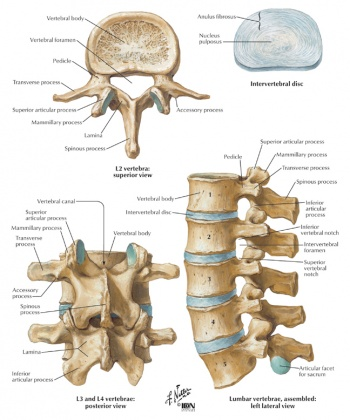
\includegraphics[scale=0.5]{cslt/lumbar_ver.jpg}
        \caption{Đốt sống}
        \label{fig:lumbar_ver-abstract}
    \end{figure}
\textbf{Đĩa đệm (Intervertebral Disc):} Trên ảnh MRI T2-weighted, đĩa đệm khỏe mạnh có tín hiệu cao ở trung tâm (nhân nhầy - nucleus pulposus) do chứa nhiều nước, và tín hiệu thấp hơn ở vòng ngoài (vòng sợi - annulus fibrosus). Khi đĩa đệm bị thoái hóa, nó sẽ mất nước và giảm tín hiệu (đen hơn). Thoát vị đĩa đệm là hình ảnh nhân nhầy lồi ra khỏi vị trí bình thường, có thể chèn ép vào các cấu trúc thần kinh. Hình~\ref{fig:disc-abstract} minh họa hình ảnh đĩa đệm.

 \begin{figure}[H]
        \centering
        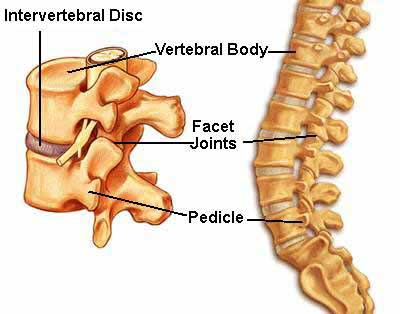
\includegraphics[scale=0.5]{cslt/disc.jpg}
        \caption{Đĩa đệm}
        \label{fig:disc-abstract}
    \end{figure}

\textbf{Tủy sống và rễ thần kinh:} Các cấu trúc này được quan sát tốt nhất trên ảnh MRI. Tủy sống nằm trong ống sống, được bao quanh bởi dịch não tủy (cerebrospinal fluid - CSF) có tín hiệu rất cao (màu trắng) trên ảnh T2-weighted. Các rễ thần kinh từ tủy sống đi ra qua các lỗ liên hợp, và sự chèn ép lên chúng bởi đĩa đệm hoặc xương là nguyên nhân phổ biến gây đau thần kinh tọa. Hình~\ref{fig:spinal-cord-abstract} minh họa tủy sống và rễ thần kinh.
\begin{figure}[H]
        \centering
        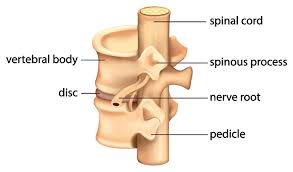
\includegraphics[scale=0.8]{cslt/spinal_cord.jpg}
        \caption{Tủy sống và rễ thần kinh}
        \label{fig:spinal-cord-abstract}
\end{figure}

\section{Mô hình Artificial Neural Network - ANN}
Mô hình Artificial Neural Network - ANN (Mạng nơ-ron nhân tạo) \cite{NN}
là mô hình tính toán được xây dựng lấy ý tưởng từ cấu trúc và cách
hoạt động của mạng nơ-ron thần kinh trong não người nhằm thực hiện một
tác vụ nào đó với tập thông tin đầu vào. Một mạng nơ-ron thần kinh được tạo nên từ nhiều nơ-ron sinh học kết
nối và hoạt động cùng nhau. Chúng hoạt động bằng cách tiếp nhận các thông tin đưa vào
từ các \textit{đuôi gai} (dendrite), tính toán và tổng hợp tại \textit{thân nơ-ron} (cell body),
sau đó lan truyền kết quả đến các nơ-ron khác thông qua \textit{sợi trục} (axon). Có thể dễ dàng rút ra nhận xét rằng \textbf{nơ-ron sinh học nhận nhiều thông
tin đầu vào nhưng chỉ đưa ra một kết quả duy nhất thôngc qua quá trình xử lý trung gian phức tạp}.

Tương tự như cách thức hoạt động nêu trên của mạng nơ-ron thần kinh,
ANN cũng được cấu thành từ nhiều nơ-ron được gọi là perceptron có cấu
trúc như Hình~\ref{fig:perceptron}. Trong đó:

\begin{itemize}
    \item[--] $x_1, x_2, x_3, ..., x_n$ lần lượt là các biến đại diện cho dữ liệu đầu vào.

    \item[--] phép cộng (\textit{summation}) và hàm kích hoạt (\textit{activation function})
là các phép tính toán và tổng hợp các thông tin dữ liệu đầu vào.

    \item[--] $w_1, w_2, w_3, ..., w_n$ là các trọng số cần phải học, đóng vai trò tham
gia quá trình tính toán và chuyển đổi các thông tin đầu vào thành
thông tin đầu ra.

    \item[--] $y$ là output của tiến trình, đại diện cho dữ liệu đầu ra.

\end{itemize}

\begin{figure}[!htb]
        \centering
        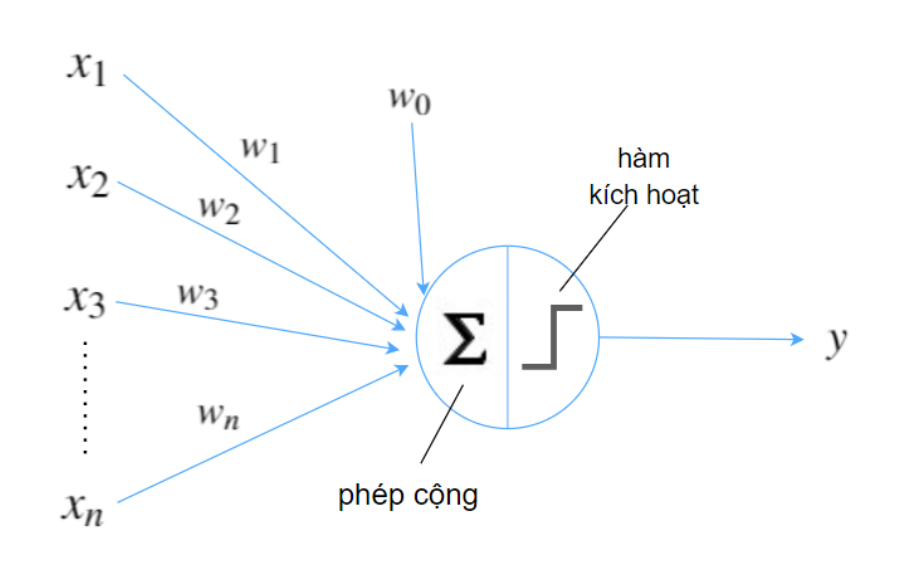
\includegraphics[width=0.75\textwidth]{cslt/perceptron.png}
        \caption{Cấu trúc của một Perceptron}
        \label{fig:perceptron}
    \end{figure}

Cụ thể hơn, phương thức tính toán và tổng hợp dữ liệu của một perceptron được mô tả theo từng bước sau:

\begin{enumerate}
    \item Perceptron
thực hiện phép cộng bằng cách tính tổng giá trị tất cả các tích số của
từng cặp dữ liệu đầu vào và giá trị trọng số tương ứng:

\begin{equation}
    a = \sum_{i = 1}^n w_ix_i + w_0
\end{equation}

    \item Kết quả $a$ của phép cộng được đưa qua một hàm kích hoạt phi
tuyến như \textit{Sigmoid, Tanh, ReLU, LeakyReLU} được minh họa ở Hình~\ref{fig:act_functions}.


\begin{figure}[!htb]
        \centering
        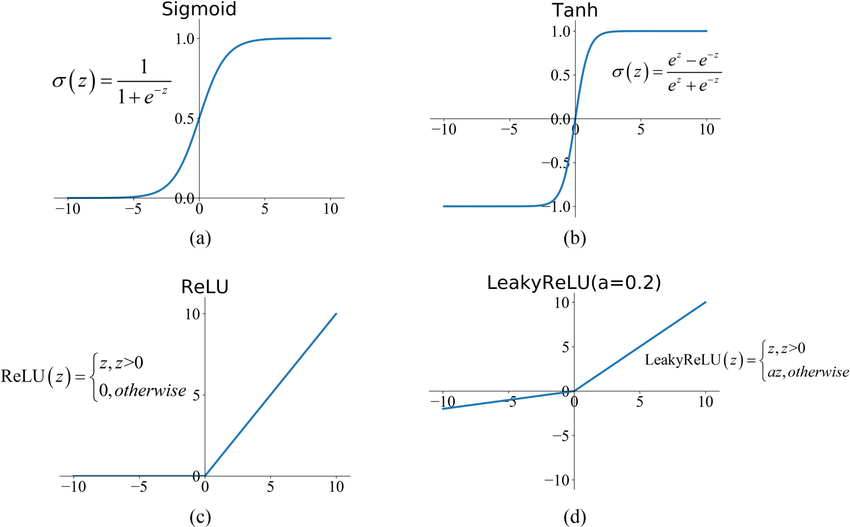
\includegraphics[width=0.85\textwidth]{cslt/act.png}
        \caption{Các hàm phi tuyến được sử dụng trong Perceptron \cite{goodfellow2016deep}.}
        \label{fig:act_functions}
    \end{figure}

    \item Sau đó, perceptron thực hiện phép so sánh giá trị nhận được từ hàm
kích hoạt \textit{f(a)} với một giá trị ngưỡng (\textit{threshold}) cho trước nhằm
xác định giá trị đầu ra $\hat{y}$ như là tín hiệu kích hoạt của perceptron.

\begin{equation}
    \hat{y} = \left\{\begin{matrix}
1   & \text{if} f(a) \geq \text{threshold}\\ 
0 &  \text{if} f(a) < \text{threshold}
\end{matrix}\right.
\end{equation}
\end{enumerate}

Bằng cách kết hợp nhiều perceptron với nhau sẽ tạo nên cấu trúc mô
hình mạng ANN. Mạng ANN bao gồm nhiều perceptron như là các nút mạng tính toán làm tăng tính phức tạp cũng như khả năng học cho mạng, các perceptron đó hình thành nên các tầng như sau:

\begin{itemize}
    \item[--] \textbf{Tầng đầu vào} (input layer): là tầng đầu tiên, thể hiện các dữ liệu đầu
vào của mô hình.
    \item[--] \textbf{Tầng ẩn} (hidden layer): là tầng nằm giữa gồm các phép tính toán nhằm
chuyển đổi dữ liệu đầu vào sang dữ liệu đầu ra. 

    \item[--] \textbf{Tầng kết quả} (output layer): là tầng cuối cùng thể hiện dữ liệu đầu ra của mạng. 
\end{itemize}

Số lượng tầng ẩn trong mô hình ANN là không giới hạn và được xác
định tùy thuộc vào bài toán cần giải quyết. Đặc biệt, khi số lượng tầng ẩn
lớn hơn 1 thì mô hình ANN được gọi là mô hình \textit{Học sâu} (Deep learning).

\section{ Mạng tích chập Convolutional Neural Network - CNN }
Mạng tích chập có 02 phần chính: \textbf{Lớp trích lọc đặc trưng của ảnh} (Conv, Relu và Pool) và \textbf{Lớp phân loại} (FC và softmax). Hình~\ref{fig:cnn} minh họa cấu trúc tổng thể của một mạng CNN cơ bản.\\
\begin{figure}[!htb]
        \centering
        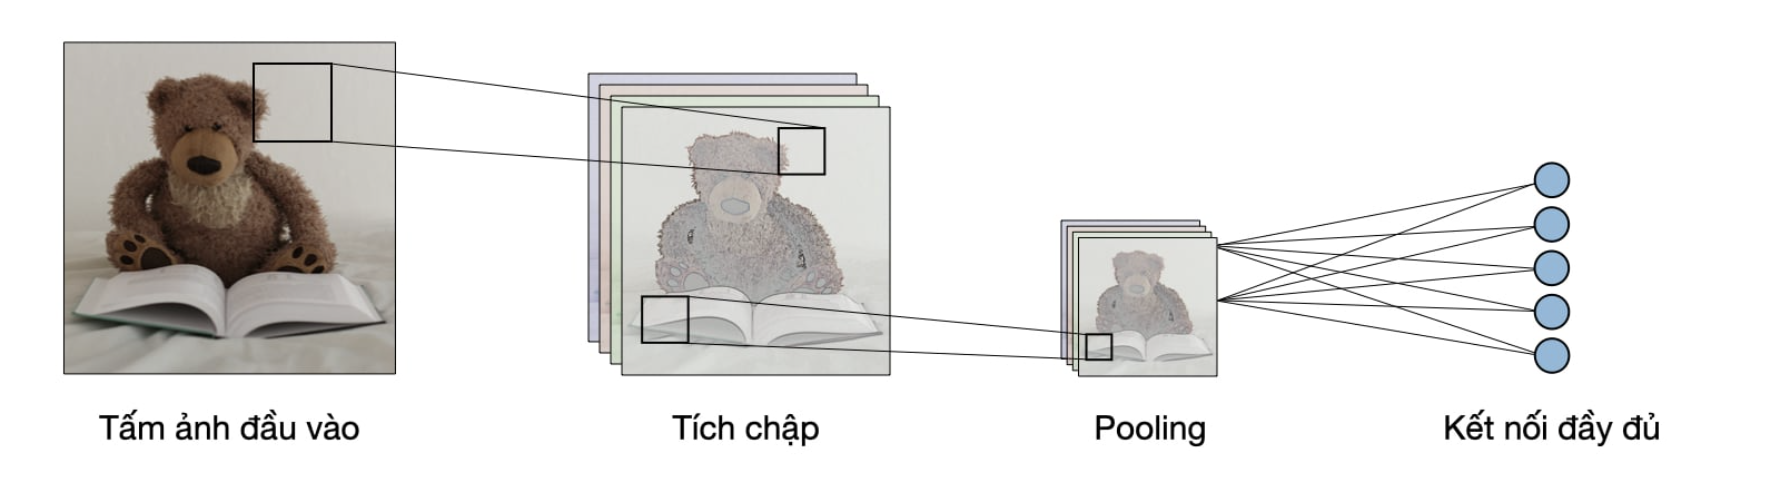
\includegraphics[width=\textwidth]{cslt/cnn.png}
        \caption{Mô hình CNN cơ bản \cite{shegaonkar2024cnn}.}
        \label{fig:cnn}
\end{figure}
Đầu vào (dữ liệu training):
\begin{itemize}
    \item Input đầu vào là một bức ảnh được biểu diển bởi ma trận pixel với kích thước: $[w \times h \times d]$
    \item W: chiều rộng
\item  H: chiều cao
\item  D: Là độ sâu, hay dễ hiểu là số lớp màu của ảnh. Ví dụ ảnh RBG sẽ là 3 lớp ảnh Đỏ, Xanh Dương, Xanh.
\end{itemize}

\textbf{Conv layer:} Mục tiêu của các lớp tích chập là trích chọn các đặc trưng của ảnh đầu vào. Ảnh đầu vào được cho qua một bộ lọc chạy dọc bức ảnh. Bộ lọc có kích thước là $m \times n$ và áp dụng phép tích vô hướng để tính toán, cho ra một giá trị duy nhất. Đầu ra của phép tích chập là một tập các giá trị ảnh được gọi là mạng đặc trưng (features map).\\

Phép tích chập đơn giản là phép tìm biên ảnh. Sau khi cho qua bộ lọc nó sẽ làm hiện lên các đặc trưng của đối tượng trong ảnh như đường vẽ xung quanh đối tượng, các góc cạnh,v.v.., và các layer tiếp theo sẽ lại trích xuất tiếp các đặc trưng của đặc trưng của các đối tượng đó, việc có nhiều layer như vậy cho phép chúng ta chia nhỏ đặc trưng của ảnh tới mức nhỏ nhất có thể.\\

\textbf{ReLU layer:} ReLU layer áp dụng các kích hoạt (activation function) max(0,x) lên đầu ra của Conv Layer, có tác dụng đưa các giá trị âm về thành 0. Layer này không thay đổi kích thước của ảnh và không có thêm bất kì tham số nào. Mục đích của lớp ReLu là đưa ảnh một mức ngưỡng, ở đây là 0. Để loại bỏ các giá trị âm không cần thiết mà có thể sẽ ảnh hưởng cho việc tính toán ở các layer sau đó.\\

\textbf{Pool layer:} Pool Layer thực hiện chức năng làm giảm chiều không gian của đầu và giảm độ phức tạp tính toán của model ngoài ra Pool Layer còn giúp kiểm soát hiện tượng overffiting. Thông thường, Pool layer có nhiều hình thức khác nhau phù hợp cho nhiều bài toán, tuy nhiên Max Pooling là được sử dụng nhiều vào phổ biến hơn cả với ý tưởng cũng rất sát với thực tế con người đó là: Giữ lại chi tiết quan trọng hay hiểu ở trong bài toán này chính giữ lại pixel có giá trị lớn nhất.\\

\textbf{Fully connected layer (FC):} Tên tiếng việt là Mạng liên kết đầy đủ. Tại lớp mạng này, mỗi một nơ-ron của layer này sẽ liên kết tới mọi nơ-ron của lớp khác. Để đưa ảnh từ các layer trước vào mạng này, buộc phải dàn phẳng bức ảnh ra thành 1 vector thay vì là mảng nhiều chiều như trước. Tại layer cuối cùng sẽ sử dụng 1 hàm kinh điển trong học máy softmax để phân loại đối tượng dựa vào vector đặc trưng đã được tính toán của các lớp trước đó.
\section{Kiến trúc Encoder-Decoder}
Kiến trúc Encoder-Decoder là một mô hình mạng nơ-ron được thiết kế để giải quyết các bài toán \textbf{chuỗi-đến-chuỗi (sequence-to-sequence - Seq2Seq)}, nơi độ dài của chuỗi đầu vào và chuỗi đầu ra có thể khác nhau. Mô hình này đã trở thành nền tảng cho nhiều ứng dụng đột phá trong xử lý ngôn ngữ tự nhiên như dịch máy, tóm tắt văn bản, và trả lời câu hỏi \cite{sutskever2014seq2seq, cho2014learning}. Hình~\ref{fig:en-de-abstract} minh họa kiến trúc Encoder-Decoder tổng quát.

\begin{figure}[!htb]
        \centering
        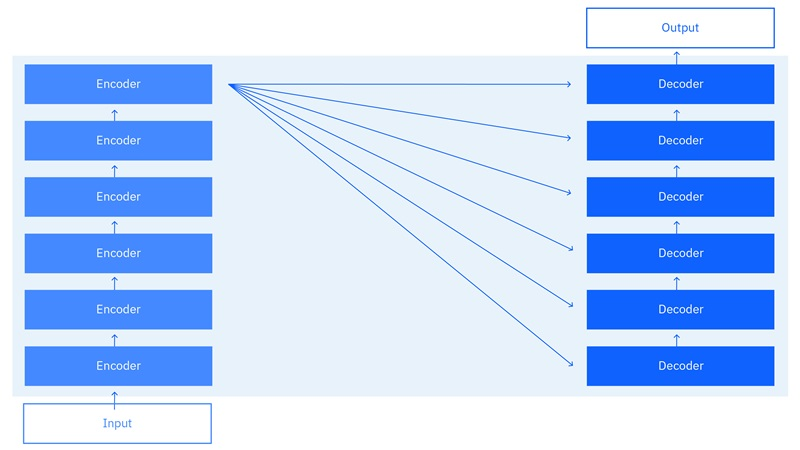
\includegraphics[width=\textwidth]{cslt/en-de.png}
        \caption{Kiến trúc Encoder-Decoder \cite{ibm_encoderdecoder}.}
        \label{fig:en-de-abstract}
\end{figure}

Về cơ bản, kiến trúc này bao gồm hai thành phần chính: \textbf{Encoder (Bộ mã hóa)} và \textbf{Decoder (Bộ giải mã)}, thường được xây dựng từ các mạng nơ-ron hồi quy (RNN), đặc biệt là LSTM (Long Short-Term Memory) hoặc GRU (Gated Recurrent Unit).



\subsection{Encoder}
Nhiệm vụ của Encoder là đọc và "hiểu" chuỗi đầu vào, sau đó nén toàn bộ thông tin của chuỗi đó thành một vector có kích thước cố định, được gọi là \textbf{vector ngữ cảnh (context vector)} hoặc "vector tư tưởng" (thought vector).

Quá trình này diễn ra tuần tự qua từng phần tử của chuỗi đầu vào.
\begin{itemize}
    \item Cho một chuỗi đầu vào $X = (x_1, x_2, \dots, x_T)$, tại mỗi bước thời gian $t$, mạng RNN của Encoder sẽ cập nhật trạng thái ẩn (hidden state) $h_t$ dựa trên phần tử đầu vào $x_t$ và trạng thái ẩn của bước trước đó $h_{t-1}$.
    \item Công thức cập nhật trạng thái ẩn có thể được biểu diễn tổng quát như sau:
    \begin{equation}
        h_t = f(W_{hh}h_{t-1} + W_{xh}x_t)
    \end{equation}
    Trong đó, $f$ là một hàm phi tuyến tính (ví dụ như hàm kích hoạt của LSTM hoặc GRU), $W_{hh}$ và $W_{xh}$ là các ma trận trọng số được huấn luyện.
    \item Sau khi xử lý toàn bộ chuỗi đầu vào qua $T$ bước, trạng thái ẩn cuối cùng $h_T$ chính là vector ngữ cảnh $C$. Vector này được kỳ vọng sẽ chứa đựng tóm tắt toàn bộ ý nghĩa của chuỗi đầu vào.
    \begin{equation}
        C = h_T
    \end{equation}
\end{itemize}

\subsection{Decoder}
Nhiệm vụ của Decoder là nhận vector ngữ cảnh $C$ từ Encoder và tạo ra chuỗi đầu ra $Y = (y_1, y_2, \dots, y_{T'})$.

\begin{itemize}
    \item Decoder cũng là một mạng RNN. Trạng thái ẩn ban đầu của nó, $s_0$, được khởi tạo bằng chính vector ngữ cảnh $C$ từ Encoder.
    \begin{equation}
        s_0 = C
    \end{equation}
    \item Tại mỗi bước thời gian $t$, Decoder sẽ tạo ra một phần tử $y_t$ của chuỗi đầu ra. Quá trình này có tính tự hồi quy (auto-regressive), nghĩa là đầu ra của bước trước $y_{t-1}$ sẽ được dùng làm đầu vào cho bước hiện tại $t$.
    \item Trạng thái ẩn $s_t$ của Decoder được cập nhật như sau:
    \begin{equation}
        s_t = g(W_{ss}s_{t-1} + W_{ys}y_{t-1})
    \end{equation}
    Trong đó, $g$ là hàm kích hoạt của RNN trong Decoder, $W_{ss}$ và $W_{ys}$ là các ma trận trọng số.
    \item Từ trạng thái ẩn $s_t$, mô hình sẽ dự đoán xác suất của từ tiếp theo trong chuỗi đầu ra thông qua một lớp softmax trên toàn bộ bộ từ vựng:
    \begin{equation}
        P(y_t | y_1, \dots, y_{t-1}, C) = \text{softmax}(W_{sy}s_t)
    \end{equation}
\end{itemize}

\subsection{Cơ chế tập trung}
Kiến trúc Encoder-Decoder cơ bản có một hạn chế lớn: nó phải nén toàn bộ thông tin của chuỗi đầu vào vào một vector ngữ cảnh $C$ có kích thước cố định. Đây trở thành một \textbf{"nút thắt cổ chai" (bottleneck)} thông tin, đặc biệt với các chuỗi đầu vào dài, khiến mô hình khó có thể ghi nhớ các chi tiết ở phần đầu của chuỗi.

Để giải quyết vấn đề này, \textbf{cơ chế Tập trung (Attention Mechanism)} đã được giới thiệu. Thay vì chỉ sử dụng trạng thái ẩn cuối cùng của Encoder, cơ chế attention cho phép Decoder tại mỗi bước giải mã có thể "nhìn lại" và tập trung vào tất cả các trạng thái ẩn của Encoder ($h_1, h_2, \dots, h_T$).
\begin{itemize}
    \item Tại mỗi bước tạo ra đầu ra $y_i$, Decoder sẽ tính toán một bộ "trọng số tập trung" $\alpha_{ij}$ cho mỗi trạng thái ẩn $h_j$ của Encoder. Trọng số này cho biết mức độ quan trọng của từ đầu vào thứ $j$ đối với việc tạo ra từ đầu ra thứ $i$.
    \item Một vector ngữ cảnh động $c_i$ được tính bằng tổng có trọng số của tất cả các trạng thái ẩn của Encoder:
    \begin{equation}
        c_i = \sum_{j=1}^{T} \alpha_{ij} h_j
    \end{equation}
    \item Vector ngữ cảnh động $c_i$ này sau đó được sử dụng để dự đoán đầu ra $y_i$. Bằng cách này, mô hình có thể tập trung vào các phần phù hợp của chuỗi đầu vào khi tạo ra từng phần của chuỗi đầu ra, giúp cải thiện đáng kể hiệu suất, đặc biệt là với các chuỗi dài.
\end{itemize}

\section{Kiến trúc U-Net}
U-Net là một kiến trúc mạng nơ-ron tích chập (CNN) được thiết kế đặc biệt cho bài toán \textbf{phân vùng ảnh y tế (biomedical image segmentation)}, được giới thiệu lần đầu bởi Ronneberger và cộng sự 
\cite{ronneberger2015unet}. Tên gọi "U-Net" xuất phát từ hình dạng chữ U đặc trưng của kiến trúc này (Hình~\ref{fig:unet}). Về bản chất, U-Net là một mô hình \textbf{Encoder-Decoder} được cải tiến, bao gồm hai phần chính: một \textbf{đường đi xuống (contracting path)} để nắm bắt ngữ cảnh và một \textbf{đường đi lên (expansive path)} để tái tạo ảnh và định vị chính xác.

\begin{figure}[!htb]
        \centering
        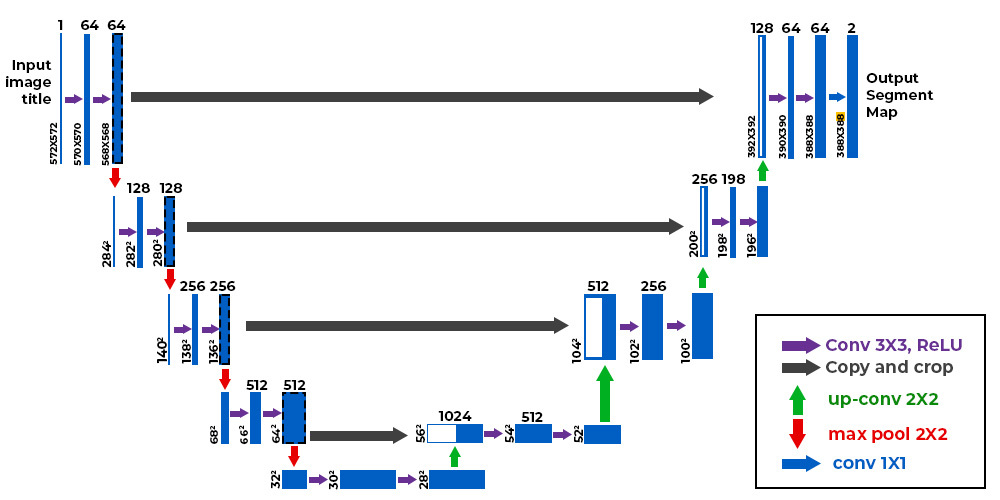
\includegraphics[width=\textwidth]{cslt/unet-arch.jpeg}
        \caption{Kiến trúc U-Net \cite{gfg_unet}.}
        \label{fig:unet}
\end{figure}

Phần đầu tiên, \textbf{đường đi xuống (Encoder)}, hoạt động như một bộ trích xuất đặc trưng. Nó bao gồm các khối lặp lại, mỗi khối chứa hai lớp tích chập 3x3 (theo sau là hàm kích hoạt ReLU) và một lớp gộp cực đại 2x2 (max pooling). Quá trình này giúp giảm dần kích thước không gian của ảnh (downsampling) trong khi tăng dần số lượng kênh đặc trưng. Nhờ đó, mô hình có thể học được các thông tin ngữ cảnh phức tạp và trừu tượng của ảnh đầu vào, hay nói cách khác là "hiểu được cái gì" đang có trong ảnh, nhưng lại làm mất đi thông tin về vị trí chính xác.

Đối xứng với nó là \textbf{đường đi lên (Decoder)}. Nhiệm vụ của phần này là xây dựng lại một bản đồ phân vùng có độ phân giải cao từ các đặc trưng đã được mã hóa. Tại mỗi bước, nó sử dụng một lớp tích chập chuyển vị 2x2 (transposed convolution) để tăng kích thước không gian lên gấp đôi (upsampling). Điểm cải tiến cốt lõi và làm nên sức mạnh của U-Net chính là các \textbf{kết nối tắt (skip connections)}. Tại mỗi bước đi lên, bản đồ đặc trưng sau khi được tăng kích thước sẽ được ghép (concatenate) với bản đồ đặc trưng có cùng độ phân giải từ đường đi xuống tương ứng. Các kết nối tắt này cho phép mô hình kết hợp thông tin ngữ cảnh trừu tượng từ Decoder với thông tin không gian chi tiết, có độ phân giải cao từ Encoder. Sự kết hợp này giúp giải quyết vấn đề mất mát thông tin vị trí, cho phép mô hình định vị các đối tượng một cách cực kỳ chính xác – tức là "biết được nó nằm ở đâu". Sau khi ghép, khối này tiếp tục được xử lý qua hai lớp tích chập 3x3.

Cuối cùng, một lớp tích chập 1x1 được sử dụng ở lớp cuối cùng để ánh xạ bản đồ đặc trưng đa kênh thành bản đồ phân vùng cuối cùng với số kênh tương ứng với số lớp đối tượng cần phân loại.
\section{Context-Aware Transformers}
Trong khi các mạng CNN (như U-Net) rất mạnh trong việc trích xuất các đặc trưng cục bộ chi tiết, chúng lại gặp khó khăn trong việc nắm bắt các mối quan hệ ngữ cảnh ở phạm vi xa  trong một tấm ảnh. Ngược lại, kiến trúc Transformer, vốn thành công trong xử lý ngôn ngữ, lại có khả năng mô hình hóa các mối quan hệ toàn cục nhưng có thể bỏ qua các chi tiết kết cấu ở mức độ pixel.

Để kết hợp ưu điểm của cả hai phương pháp, kiến trúc \textbf{Context-Aware Transformers} đã được đề xuất, đặc biệt cho các bài toán phân vùng y tế, nơi cả ngữ cảnh toàn cục và chi tiết cục bộ đều cực kỳ quan trọng \cite{windsor2022context}. Ý tưởng cốt lõi là tạo ra một mô hình "nhận thức được ngữ cảnh" bằng cách kết hợp song song hai luồng xử lý thông tin.

Kiến trúc này thường bao gồm một bộ mã hóa \textbf{hai nhánh}:
\begin{enumerate}
    \item \textbf{Nhánh nhận thức cục bộ (Local-Aware Branch):} Thường là một mạng CNN (ví dụ: một phần của kiến trúc ResNet). Nhánh này có nhiệm vụ xử lý ảnh đầu vào và trích xuất các bản đồ đặc trưng (feature maps) giàu thông tin về kết cấu, hình dạng và các chi tiết ở phạm vi hẹp. Đây là thế mạnh truyền thống của CNN.

    \item \textbf{Nhánh nhận thức toàn cục (Global-Aware Branch):} Đây là một kiến trúc dựa trên Transformer (cụ thể là Vision Transformer - ViT). Ảnh đầu vào được chia thành các "mảnh" (patches) nhỏ, sau đó được "dát phẳng" và đưa vào các khối Transformer Encoder. Nhờ cơ chế tự tập trung (self-attention), nhánh này có thể học được mối tương quan giữa tất cả các cặp mảnh ảnh, bất kể chúng nằm ở đâu. Điều này cho phép mô hình nắm bắt được ngữ cảnh tổng thể của bức ảnh.
\end{enumerate}

Điểm mấu chốt của mô hình là một \textbf{mô-đun hợp nhất (fusion module)} được thiết kế để kết hợp hiệu quả thông tin từ hai nhánh trên. Các đặc trưng cục bộ chi tiết từ nhánh CNN sẽ được làm giàu thêm bằng các thông tin ngữ cảnh toàn cục từ nhánh Transformer. Biểu diễn kết hợp này sau đó được đưa vào một bộ giải mã, thường có cấu trúc tương tự như U-Net, để tái tạo lại bản đồ phân vùng cuối cùng.

Bằng cách này, Context-Aware Transformer có thể vừa tận dụng khả năng nắm bắt chi tiết tinh vi của CNN, vừa khai thác được khả năng hiểu ngữ cảnh toàn cục của Transformer, từ đó cải thiện đáng kể độ chính xác trong các tác vụ phân vùng phức tạp.

\section{Cơ chế attention CBAM (Convolutional block attention module)}
Mặc dù mạng tích chập (CNN) trích xuất đặc trưng tốt từ ảnh, không phải mọi kênh đặc trưng và mọi vị trí không gian đều mang thông tin hữu ích như nhau cho bài toán phân loại. Đặc biệt với ảnh y tế, vùng bệnh lý (ví dụ vùng thoát vị đĩa đệm, vùng hẹp ống sống) thường chiếm tỉ lệ rất nhỏ so với toàn bộ khối ảnh đầu vào. \textbf{CBAM (Convolutional Block Attention Module)} được Woo và cộng sự \cite{woo2018cbam} giới thiệu năm 2018 là một mô-đun chú ý nhẹ, có thể chèn vào bất kì vị trí nào của một CNN, giúp mô hình tự động học cách "tập trung" vào các kênh đặc trưng và các vị trí không gian quan trọng nhất.

CBAM bao gồm hai phần tuần tự: \textbf{chú ý theo kênh} (Channel Attention) và \textbf{chú ý theo không gian} (Spatial Attention). Với đầu vào là một tensor đặc trưng $F$ có kích thước $C \times H \times W$, phần Channel Attention tính một vector chú ý theo kênh $M_c$ kích thước $C \times 1 \times 1$ qua các bước:
\begin{itemize}
    \item Áp dụng đồng thời Average Pooling và Max Pooling trên chiều không gian, thu được hai vector kích thước $C \times 1 \times 1$.
    \item Đưa hai vector này qua cùng một mạng MLP hai lớp (chia sẻ trọng số) để học các quan hệ phi tuyến giữa các kênh.
    \item Cộng hai đầu ra và đưa qua hàm sigmoid để chuẩn hóa về khoảng $[0, 1]$.
\end{itemize}

Công thức được viết tóm tắt như sau:
\begin{equation}
M_c(F) = \sigma\left(\text{MLP}(\text{AvgPool}(F)) + \text{MLP}(\text{MaxPool}(F))\right)
\end{equation}

Vector $M_c$ sau đó được nhân theo từng kênh với $F$ ban đầu để khuếch đại các kênh quan trọng và làm yếu các kênh ít liên quan: $F' = M_c(F) \otimes F$.

Phần Spatial Attention nhận đầu ra $F'$ từ bước trên và sinh một mặt nạ chú ý theo không gian $M_s$ kích thước $1 \times H \times W$:
\begin{itemize}
    \item Áp dụng Average Pooling và Max Pooling theo chiều kênh, thu được hai feature map kích thước $1 \times H \times W$.
    \item Ghép hai feature map này theo chiều kênh thành tensor kích thước $2 \times H \times W$.
    \item Đưa qua một lớp convolution $7 \times 7$ (filter size lớn để bắt được ngữ cảnh không gian rộng), sau đó qua hàm sigmoid.
\end{itemize}

Công thức:
\begin{equation}
M_s(F') = \sigma\left(\text{Conv}_{7\times 7}\left([\text{AvgPool}(F'); \text{MaxPool}(F')]\right)\right)
\end{equation}

Đầu ra cuối cùng là $F'' = M_s(F') \otimes F'$.

CBAM rất phù hợp cho bài toán ảnh y tế vì hai lý do chính. Thứ nhất, số tham số mà CBAM thêm vào rất ít, chỉ vài chục nghìn so với hàng chục triệu của backbone CNN, nên không gây overfitting trên các dataset y tế thường có quy mô nhỏ. Thứ hai, cơ chế chú ý ngầm cho phép mô hình học cách "nhìn vào đâu" mà không cần thông tin định vị thủ công (ví dụ bounding box hay mặt nạ phân vùng). Trong báo cáo này, CBAM được chèn sau mỗi stage của 3D ResNet-34 (4 stages tương ứng 64, 128, 256, 512 kênh) trong nhánh trainable của kiến trúc Hybrid đề xuất ở Chương 4.


\section{Các mô hình nền tảng trong ảnh y tế}

\subsection{Mô hình Segment Anything (SAM)}
Mô hình Segment Anything (SAM) được giới thiệu là một mô hình nền tảng cho bài toán phân vùng ảnh, nổi bật với khả năng khái quát hóa zero-shot thông qua kiến trúc có thể điều khiển bằng gợi ý (promptable architecture). Kiến trúc của SAM bao gồm ba thành phần chính: bộ mã hóa hình ảnh mạnh mẽ để trích xuất đặc trưng, bộ mã hóa gợi ý linh hoạt để xử lý các đầu vào như điểm hoặc hộp giới hạn, và bộ giải mã mặt nạ hạng nhẹ để tạo ra kết quả phân vùng \cite{kirillov2023sam}.

Trong lĩnh vực chẩn đoán hình ảnh, SAM cho phép thực hiện phân vùng tương tác mà không cần huấn luyện lại trên các tập dữ liệu mới. Tuy nhiên, do được huấn luyện chủ yếu trên ảnh tự nhiên, hiệu suất của SAM trên các cấu trúc y tế phức tạp có thể bị hạn chế. Để khắc phục điều này, các biến thể như MedSAM đã được phát triển bằng cách tinh chỉnh SAM trên tập dữ liệu y tế quy mô lớn, giúp mô hình thích nghi tốt hơn với các đặc điểm giải phẫu đặc thù \cite{ma2024medsam}.

\subsection{Mô hình Ngôn ngữ - Thị giác (Vision-Language Models - CLIP/BiomedCLIP)}
Các mô hình Ngôn ngữ - Thị giác, điển hình là CLIP (Contrastive Language-Image Pre-Training), đóng vai trò quan trọng trong việc liên kết thông tin đa phương thức. CLIP học cách biểu diễn hình ảnh và văn bản trong cùng một không gian nhúng chia sẻ thông qua cơ chế học tương phản, giúp tối đa hóa sự tương đồng giữa các cặp ảnh-văn bản khớp nhau và giảm thiểu sự tương đồng giữa các cặp không khớp \cite{radford2021clip}.

Mặc dù CLIP thể hiện khả năng vượt trội trên ảnh tự nhiên, việc áp dụng trực tiếp vào y tế gặp nhiều thách thức do sự phức tạp của thuật ngữ chuyên ngành và các đặc điểm hình ảnh vi mô. BiomedCLIP ra đời để giải quyết vấn đề này bằng cách huấn luyện trên quy mô lớn các cặp hình ảnh và văn bản y sinh (ví dụ: từ PubMed) \cite{zhang2024biomedclip}.

BiomedCLIP sử dụng kiến trúc chuyên biệt với Vision Transformer cho bộ mã hóa ảnh và PubMedBERT cho bộ mã hóa văn bản. Nhờ đó, mô hình có khả năng mã hóa các biểu diễn tiềm ẩn giàu ý nghĩa, giúp định vị chính xác các vùng bệnh lý và hiểu sâu sắc ngữ cảnh y khoa hơn so với mô hình CLIP tiêu chuẩn. Đây là cơ sở quan trọng để phát triển các phương pháp phân vùng zero-shot định hướng bởi văn bản \cite{zhang2024biomedclip}.